\begin{figure}[htb]
	\centering
	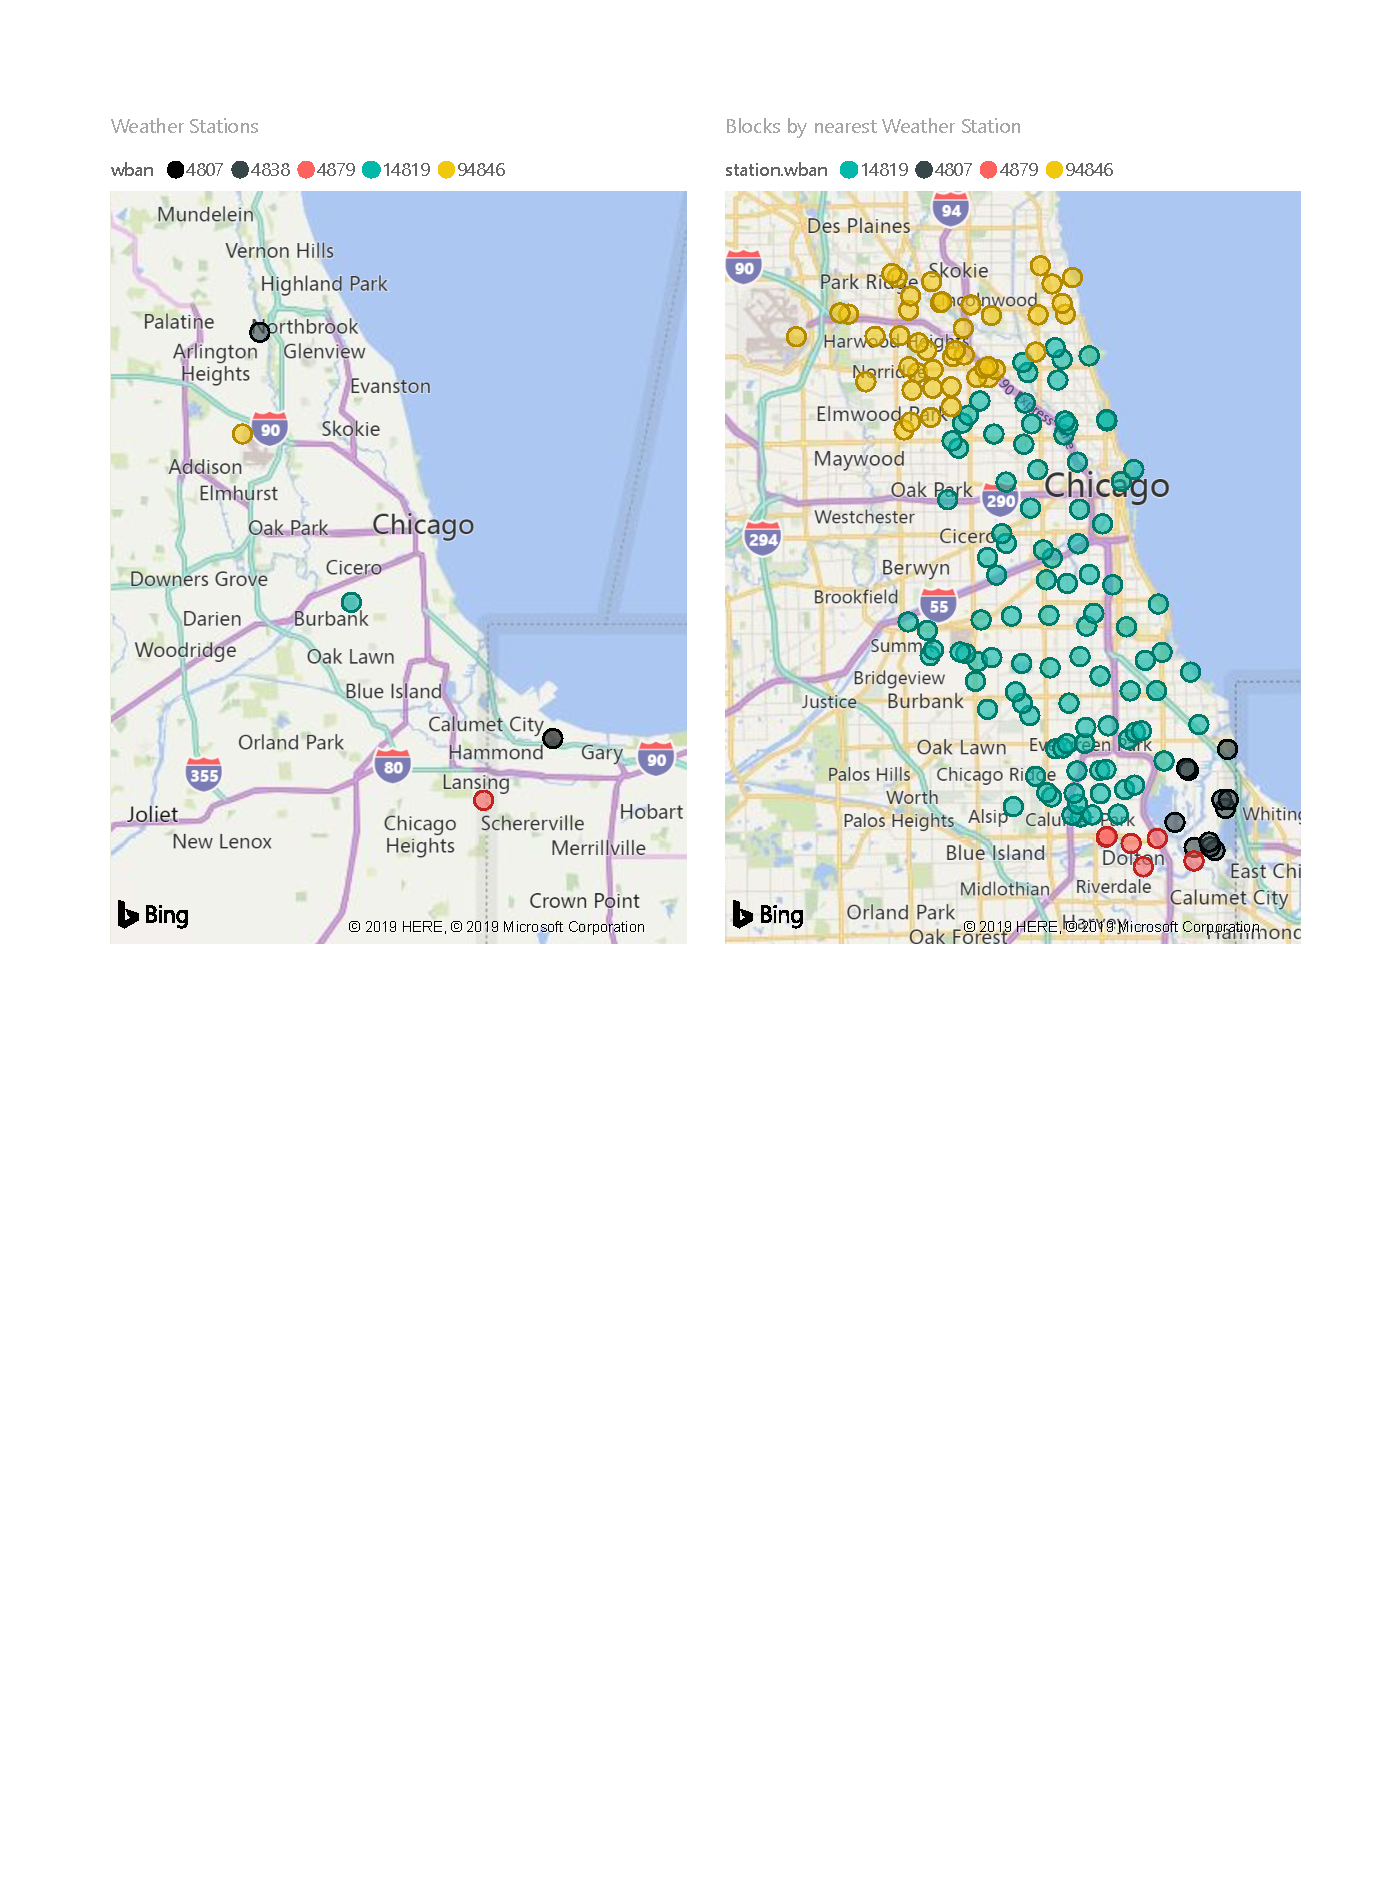
\includegraphics[width=0.4\columnwidth]{images/WeatherStations}
	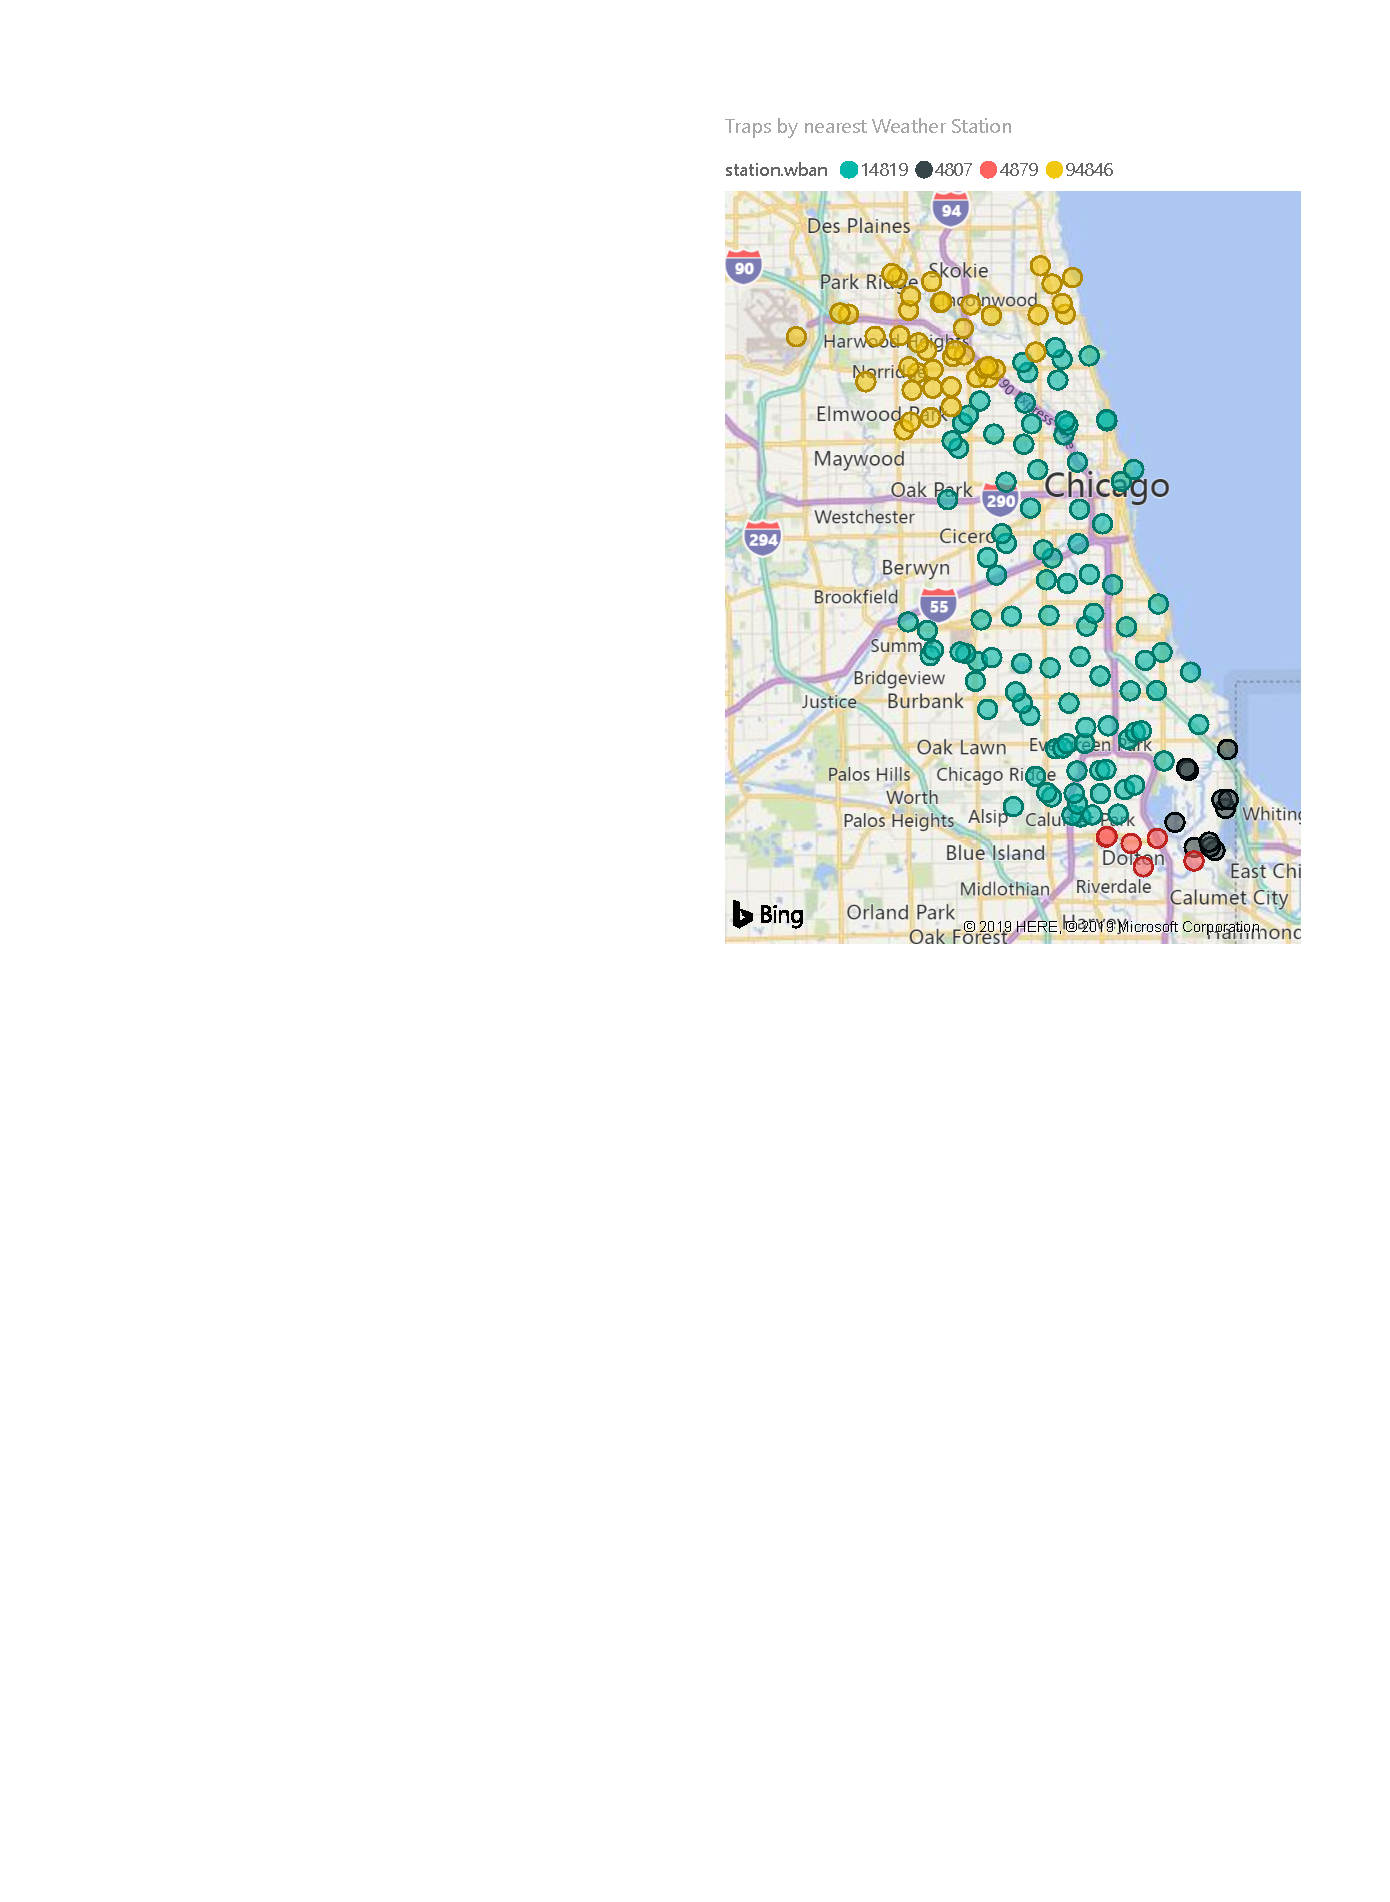
\includegraphics[width=0.4\columnwidth]{images/TrapsByNN}
	\caption{FIXME }
	\label{fig:weather-stations}
\end{figure}


Per evidenziare eventuali tendenze degli attributi, è stata effettuata 
un'analisi descrittiva sui dati integrati.


Da quest'analisi si evince che:
\begin{itemize}
	\item il 92\% dei test ha un risultato negativo;
	\item il 95\% delle trappole è di tipo Gravid;
	\item i test vengono effettuati solamente nei giorni lavorativi, in 
	particolare tra il giovedì e il venerdì;
	\item il 66\% dei blocchi ottiene i dati meteo dalla stazione Chicago 
	Midway International Airport;
	\item la media dei valori assunti dalle colonne \texttt{suspicious} è 
	0,017, valore molto buono poiché prossimo allo 0;
	\item mediamente vengono catturate 13 zanzare in ogni test.
\end{itemize} 
